\chapter{Schwarzschild black hole}
\label{s:sch}
\index{Schwarzschild!black hole}

\minitoc

\section{Introduction}

\section{Schwarzschild solution}

\section{Maximal extension}

\begin{figure}
\centerline{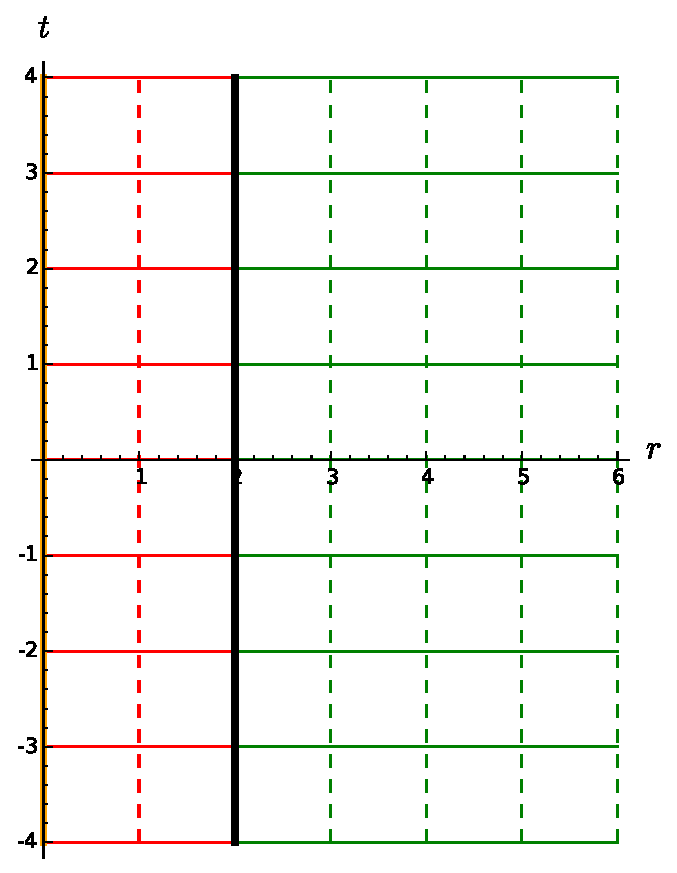
\includegraphics[height=0.37\textheight]{sch_coord_schwarz.pdf}\qquad
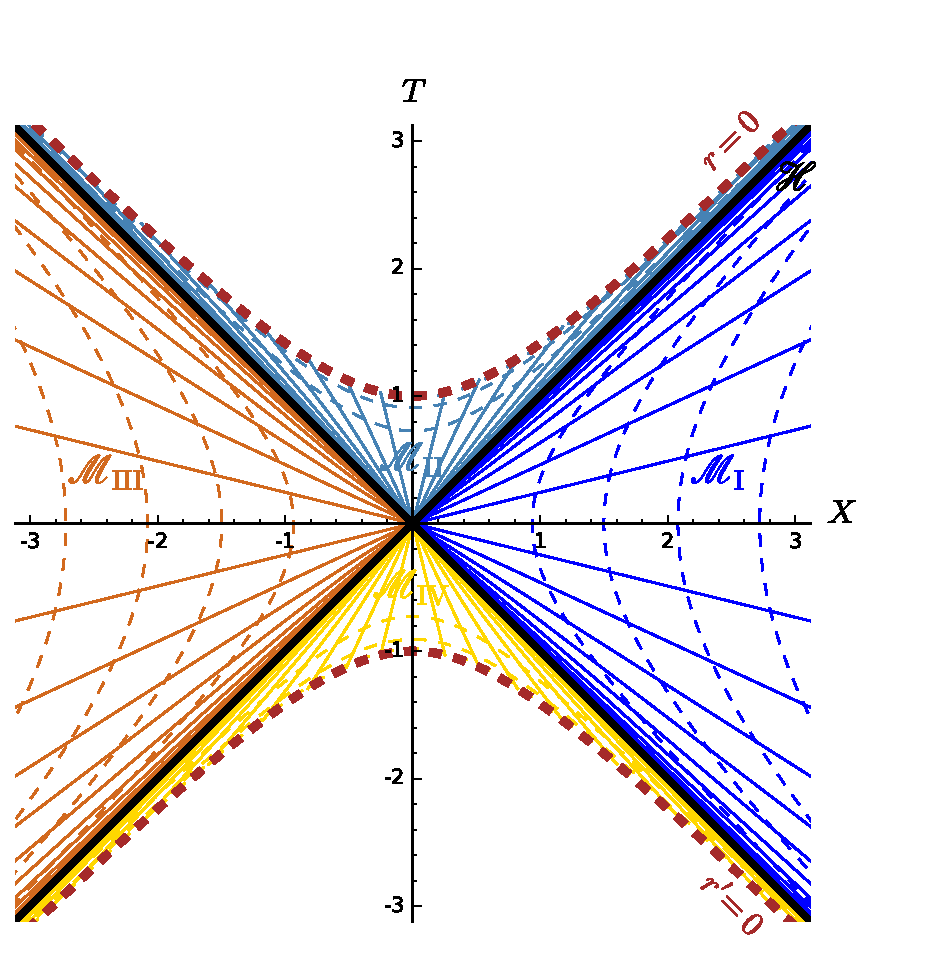
\includegraphics[height=0.37\textheight]{sch_kruskal_diag.pdf}}
\caption[]{\label{f:sch:kruskal_diag} \footnotesize
Schwarzschild spacetime depicted in Schwarzschild-Droste coordinates $(t,r)$
(left) and in Kruskal-Szekeres coordinates $(T,X)$ (right). In both figures,
green (resp. red) solid curves denote the hypersurfaces $t=\mathrm{const}$
in Region~I (resp. II), while green (resp. red) dashed curves
denote the hypersurfaces $r=\mathrm{const}$ in Region~I (resp. II).
The future and past event horizons are marked by thick black lines, while the
singularity at $r=0$ is depicted in orange. Regions III and IV are depicted
in grey and pink respectively. Note that the left figure covers only Regions I and II.}
\end{figure}

\begin{figure}
\centerline{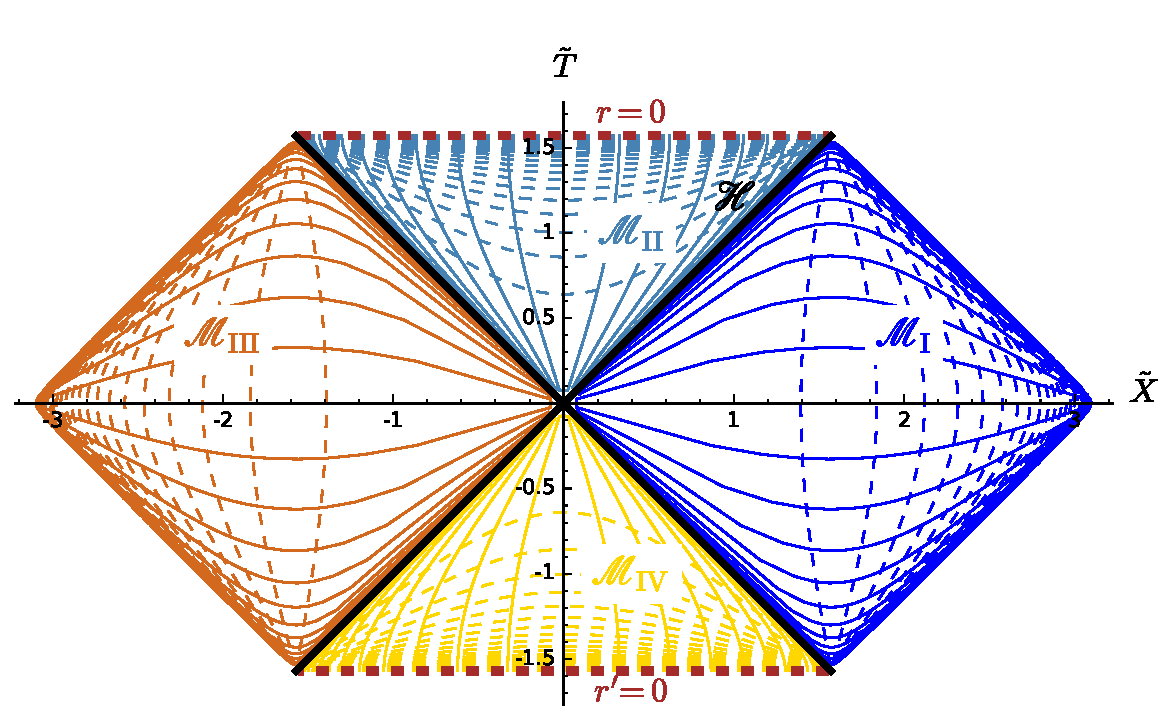
\includegraphics[width=0.9\textwidth]{sch_carter-penrose.pdf}}
\caption[]{\label{f:sch:sch_carter-penrose} \footnotesize
Schwarzschild spacetime depicted in Carter-Penrose coordinates $(\tilde{T},\tilde{X})$; the color code
is the same as in Fig.~\ref{f:sch:kruskal_diag}.
As Fig.~\ref{f:sch:kruskal_diag}, this figure has been produced with
SageManifolds (cf. Appendix~\ref{s:sam}).}
\end{figure}

